
%- Para resolver la problematica se propone una simulacion
%- una simulacion es
%- la simulacion nos puede ayudar en
%- podemos disenar la simulacion asi
%- los resultados obtenidos en la simulacion seran buen comienzo para lograr el objetivo en la vida real
\noindent
Para comenzar a abordar la problemática planteada, se propone el uso de una simulación como herramienta para
obtener resultados que puedan ser un buen punto de partida para futuras investigaciones en la vida real.
Una simulación es una representación de un sistema o proceso en un entorno controlado y artificial,
que permite estudiar y analizar el comportamiento del sistema en diferentes condiciones y escenarios.
La simulación nos puede proporcionar el comportamiento del vehículo y su entorno en situaciones de estacionamiento,
lo que nos permitirá hacer mediciones y análisis detallados de los datos obtenidos similar a como se haría en la vida real.
Además, la simulación nos brinda la flexibilidad de diseñar y modificar el entorno de estacionamiento y las condiciones de prueba

\subsection{Carla Simulator}\label{subsec:carla-simulator}
Para llevar a cabo la simulación propuesta, se utilizará: \texttt{%
    \href{https://github.com/carla-simulator/carla}{%
        CARLA Simulator}%
}
, (Car Learning to Act) un entorno de simulación de código abierto para la investigación en conducción autónoma.

CARLA incluye distribuciones urbanas, una multitud de modelos de vehículos, edificios, peatones y señales de tráfico. La plataforma de simulación admite una configuración flexible de conjuntos de sensores y proporciona señales
que pueden ser utilizadas para entrenar estrategias de conducción, tales como coordenadas GPS, velocidad, aceleración y datos detallados sobre colisiones y otras infracciones. Se puede especificar una amplia gama de condiciones ambientales, incluyendo el clima y la hora del día~\cite{dosovitskiy2017carla}.

Varias de estas condiciones ambientales se ilustran en la figura~\ref{fig:carla-simulator}.

\begin{figure}[!ht]
    \centering
    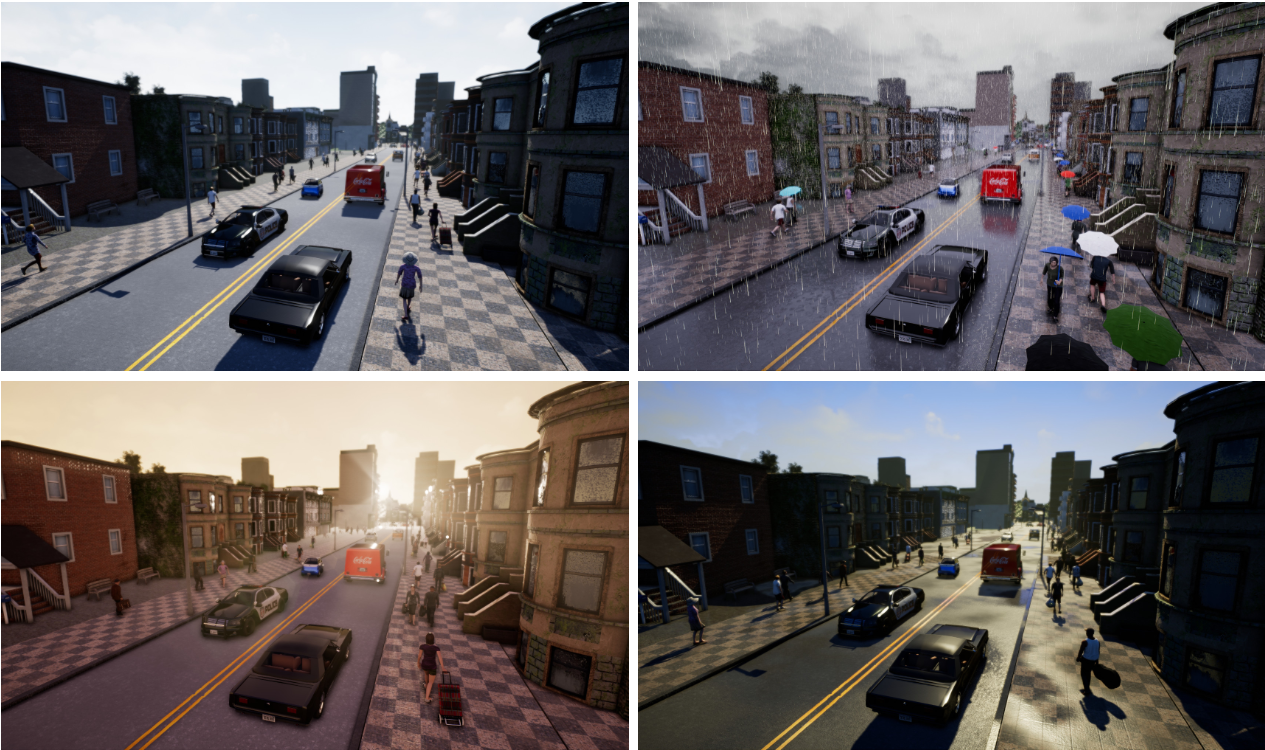
\includegraphics[width=0.9\textwidth]{img/carla_clima_example}
    \caption{Condiciones ambientales en el simulador CARLA.}
    \label{fig:carla-simulator}
\end{figure}

\subsection{Diseño del entorno de simulación}\label{subsec:simulation-design}

Para modelar el entorno de simulación, se propone un escenario de estacionamiento que incluye un vehículo y un espacio de estacionamiento.
La ubicación del vehículo, el espacio de estacionamiento y las condiciones ambientales se pueden inicializar de manera aleatoria en el simulador.
El vehículo estará equipado con sensores que proporcionarán los datos de entrada que se utilizarán para estimar la posición del vehículo con respecto al espacio de estacionamiento.
Estos sensores incluirán cámaras y sonar para capturar imágenes y distancias, respectivamente.

En la figura~\ref{fig:simulation-design} se muestra un ejemplo de cómo se podría diseñar el entorno de simulación.

\begin{figure}[!ht]
    \centering
    \begin{subfigure}{0.4\textwidth}
        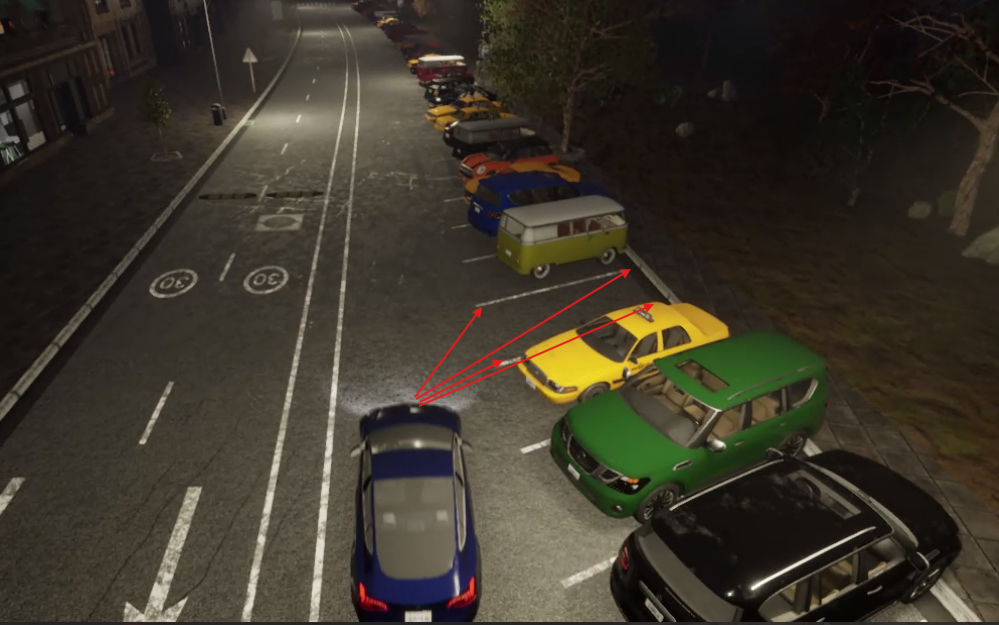
\includegraphics[width=\textwidth]{img/distances}\label {fig:distances}
    \end{subfigure}
    \begin{subfigure}{0.4\textwidth}
        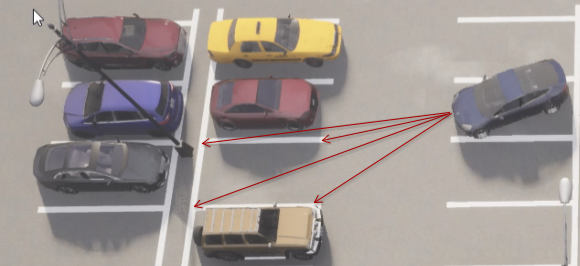
\includegraphics[width=\textwidth]{img/distances2}\label {fig:distances2}
    \end{subfigure}
    
    \caption{Diseño del entorno de simulación en CARLA.}
    \label{fig:simulation-design}
\end{figure}

\noindent
La cámara del vehículo capturará imágenes del entorno y el espacio de estacionamiento y el simulador permite ubicarla a conveniencia en el vehículo.

La ubicación de la cámara estará en la zona delantera del vehículo a una altura conocida (detrás del retrovisor). La siguiente figura ~\ref{fig:camera-view} muestra un ejemplo de como se visualiza el entorno desde la perspectiva de la cámara.

\begin{figure}[!ht]
    \centering
    \begin{subfigure}{0.4\textwidth}
        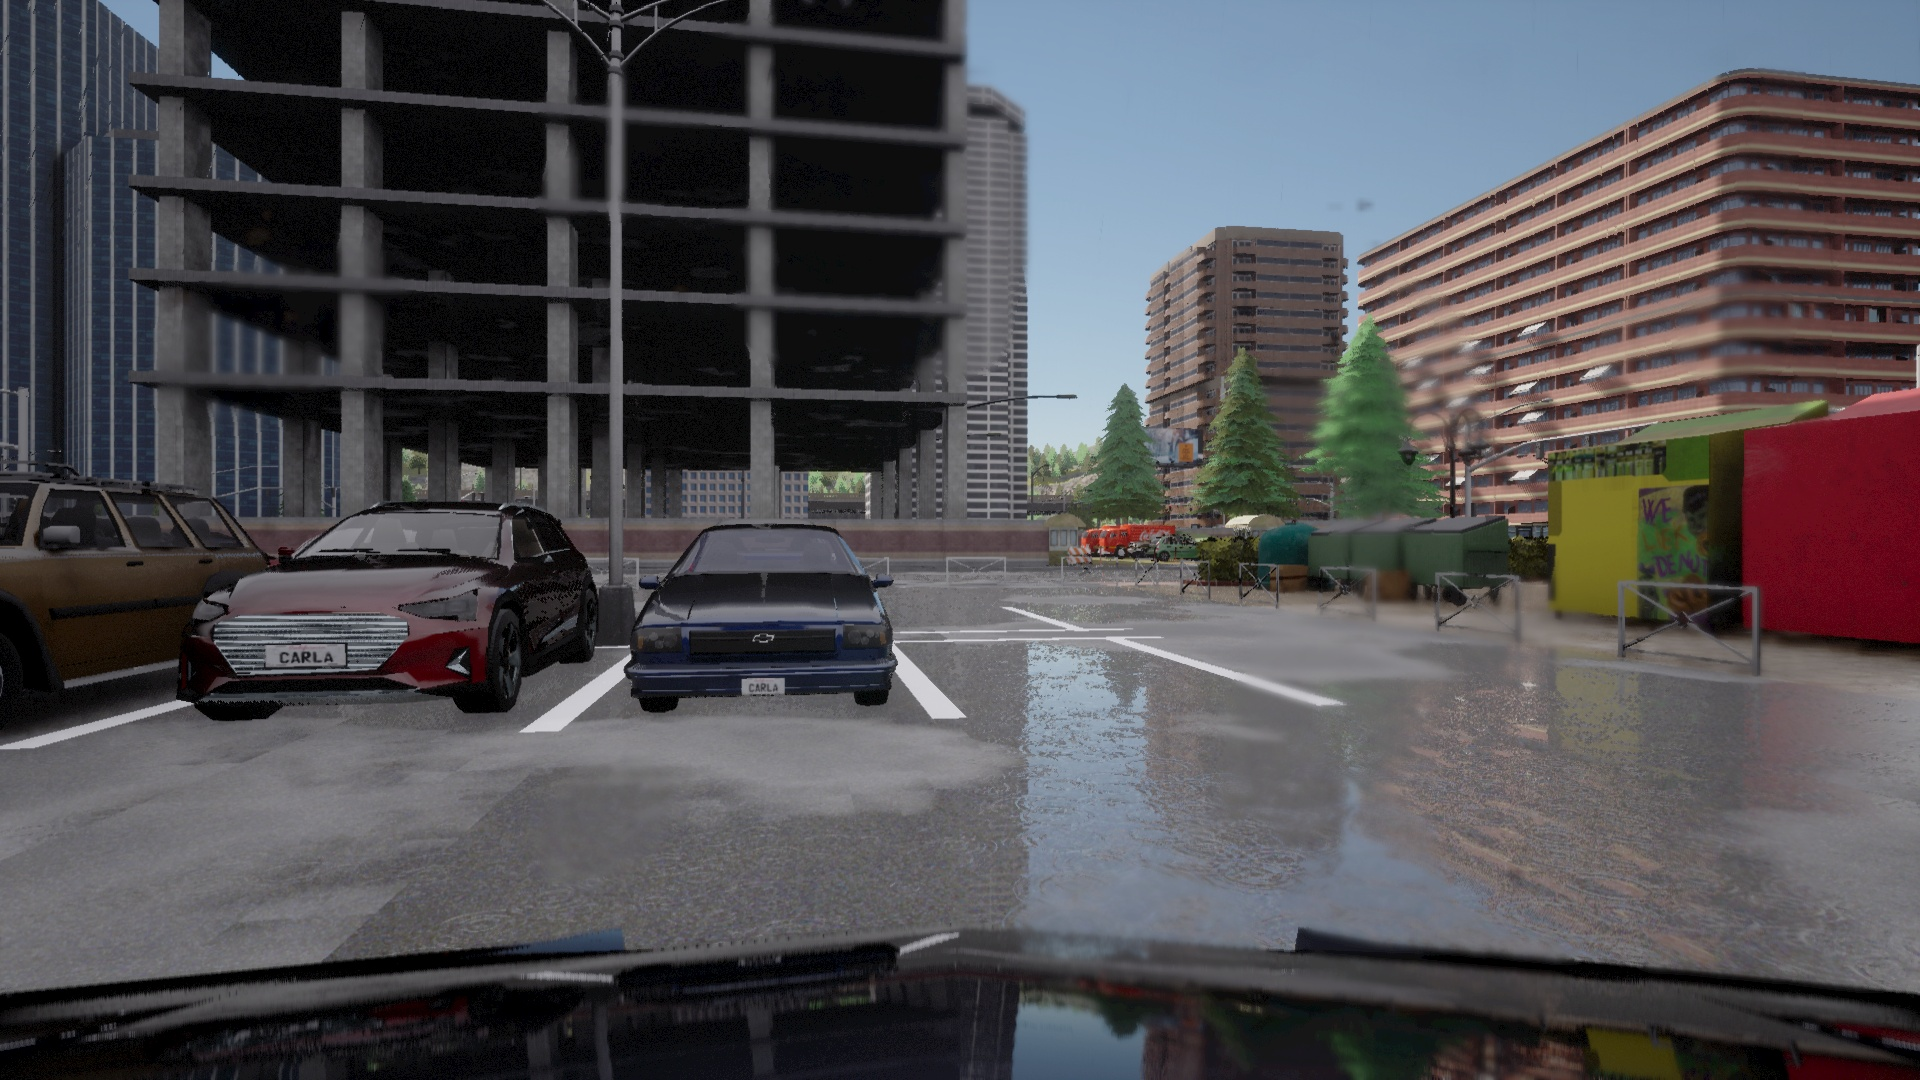
\includegraphics[width=\textwidth]{img/mirrow_camara_ex}\label {fig:camara}
    \end{subfigure}
    \begin{subfigure}{0.4\textwidth}
        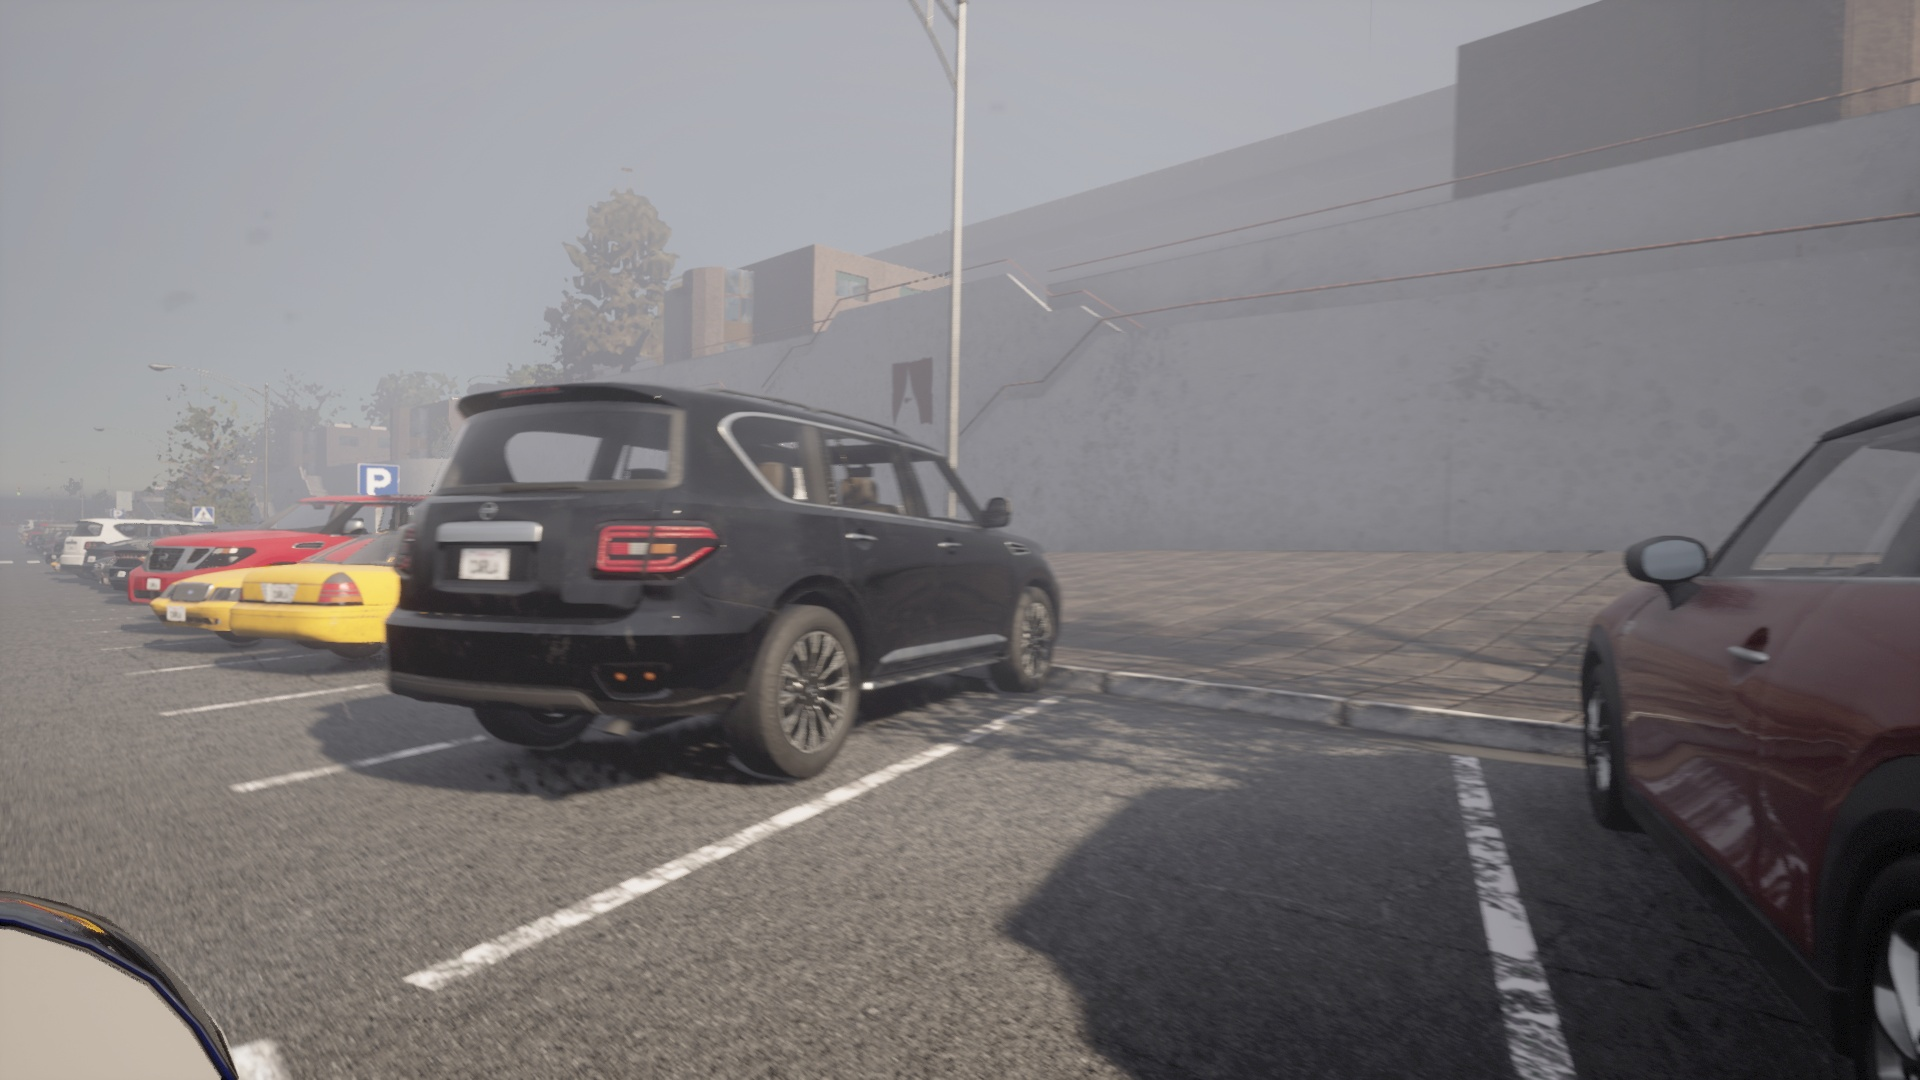
\includegraphics[width=\textwidth]{img/mirrow_camara_ex2}\label {fig:camara2}
    \end{subfigure}
    \caption{Vista de la cámara en el entorno de simulación.}
    \label{fig:camera-view}
\end{figure}




